\documentclass[11pt,a4paper]{article}

\usepackage[utf8]{inputenc}
\usepackage[T1]{fontenc}
\usepackage[spanish]{babel}
\usepackage{amsmath,amssymb}
\usepackage{graphicx}
\usepackage{geometry}
\usepackage{xcolor}
\usepackage{hyperref}
\usepackage{caption}

\geometry{margin=2.5cm}
\hypersetup{colorlinks=true, linkcolor=blue!60!black, urlcolor=blue!60!black}

\title{\textbf{De los números pares a los ceros de Riemann}\\[0.4em]
\large Un recorrido visual: primos, la función zeta y la condición de Barkhausen}
\author{Cuaderno de trabajo --- carpeta \texttt{06-grafico}}
\date{\today}

\begin{document}

\maketitle

\begin{abstract}
Este documento recorre, paso a paso y con gráficos generados numéricamente,
la relación entre dos objetos que a primera vista no tienen nada que ver: los
\emph{números primos} (que viven sobre el eje real) y los \emph{ceros no
triviales de la función zeta de Riemann} (que viven sobre la recta vertical
$\mathrm{Re}(s)=1/2$). El hilo conductor es una analogía con la \textbf{condición
de oscilación de Barkhausen}: los ceros sobre la recta $1/2$ describen un sistema
en \emph{estabilidad marginal}, que ni diverge ni se apaga, sino que oscila para
siempre. Cerramos con la \textbf{fórmula explícita de Riemann}, que muestra cómo
los ceros ``reconstruyen'' literalmente a los primos.
\end{abstract}

\tableofcontents

\section{Punto de partida: pares y primos}

Arrancamos con las dos sucesiones más básicas.

\begin{itemize}
  \item \textbf{Números pares:} generados por la fórmula $2n$. Secuencia:
  $2,4,6,8,\dots$ Todos son múltiplos de $2$. Es una progresión perfectamente
  regular.
  \item \textbf{Números primos:} naturales mayores que $1$ divisibles solo por
  $1$ y por sí mismos. Secuencia: $2,3,5,7,11,13,\dots$ A excepción del $2$
  (el único primo par), todos son impares. Su espaciado es irregular.
\end{itemize}

La Figura~\ref{fig:sucesiones} grafica los primeros $500$ términos de cada una,
con la posición $n$ en el eje horizontal y el valor en el vertical.

\begin{figure}[h]
  \centering
  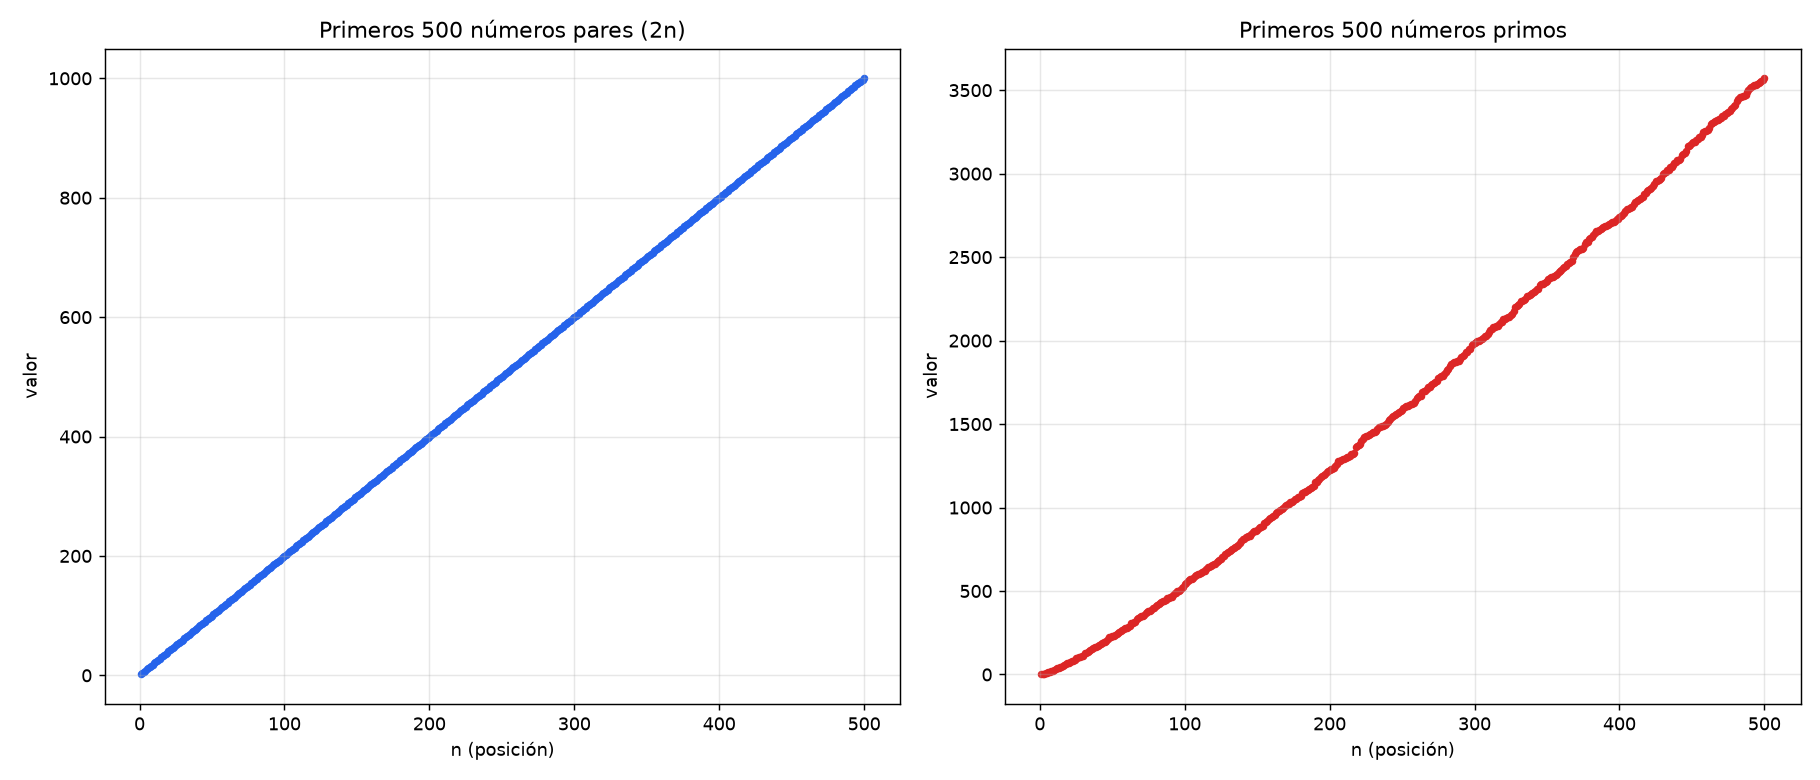
\includegraphics[width=\textwidth]{sucesiones.png}
  \caption{Primeros $500$ pares (izquierda) y primos (derecha). Los pares forman
  una recta perfecta ($2n$); los primos, una curva que se abre lentamente hacia
  arriba.}
  \label{fig:sucesiones}
\end{figure}

\section{Ampliando la escala: 10.000 términos}

Al llevar ambas sucesiones a $10.000$ términos (Figura~\ref{fig:diez_mil}), la
diferencia se acentúa: el par número $10.000$ vale $20.000$, mientras que el
primo número $10.000$ vale $104.729$ ---más de cinco veces más alto en la misma
posición. La curvatura de los primos, que refleja el
\textbf{Teorema de los Números Primos} ($p_n \sim n\ln n$), se vuelve evidente.

\begin{figure}[h]
  \centering
  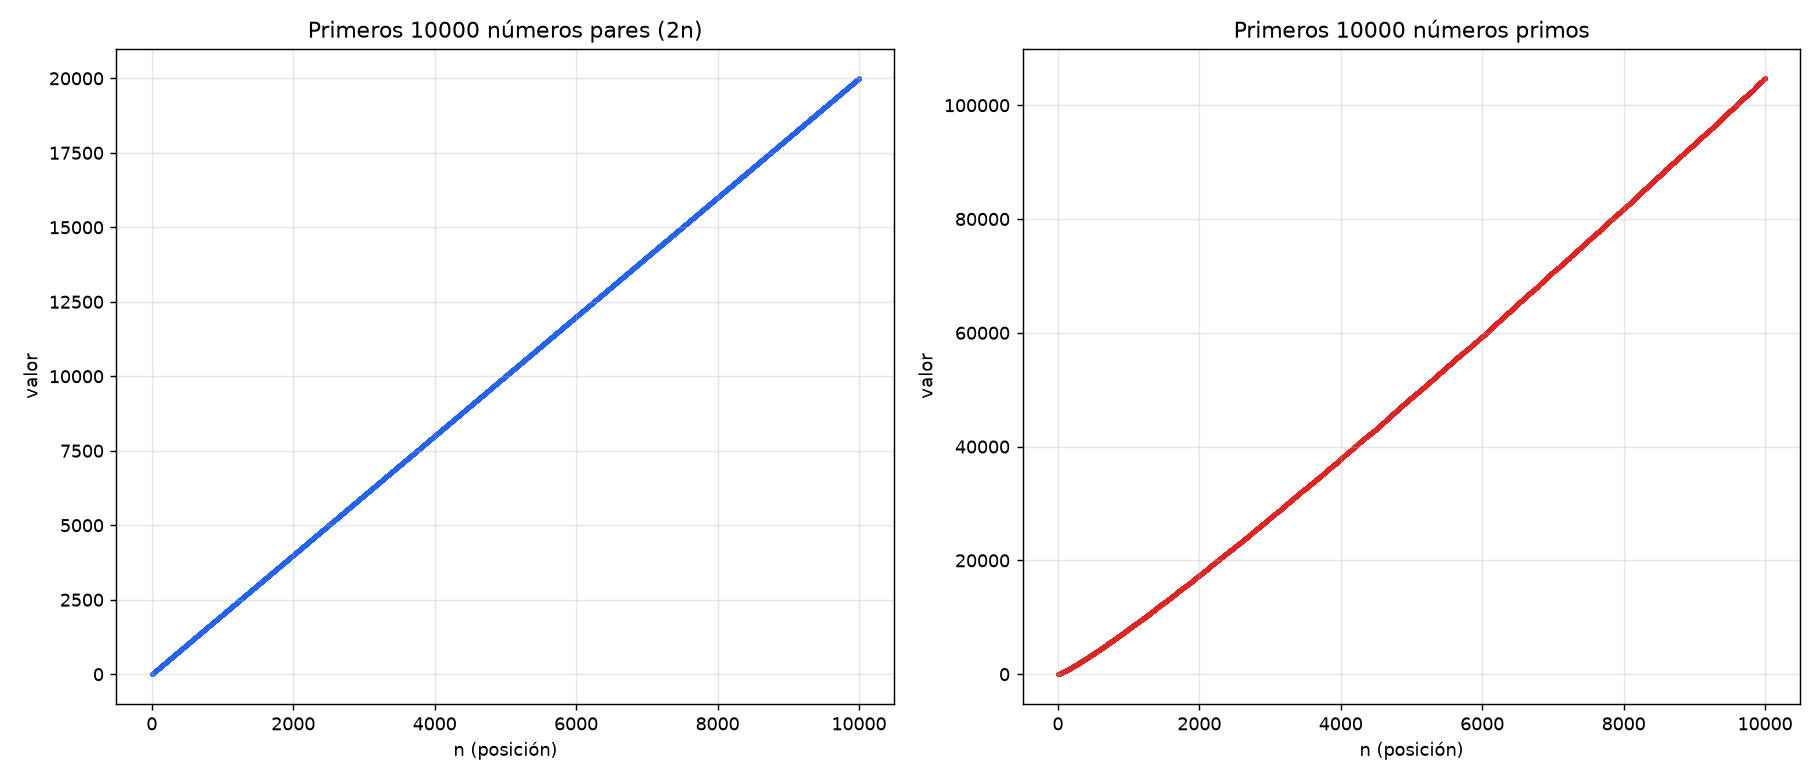
\includegraphics[width=\textwidth]{sucesiones_10000.png}
  \caption{Primeros $10.000$ pares y primos, cada uno en su propia escala.}
  \label{fig:diez_mil}
\end{figure}

\subsection{El efecto de la escala compartida}

Un detalle importante: al graficarlos por separado, cada uno usa su propia escala
vertical, lo que ``endereza'' visualmente a los primos. Al ponerlos en el
\emph{mismo plano y mismos ejes} (Figura~\ref{fig:comparacion}) se ve que los
primos crecen mucho más rápido que los pares. Añadimos además dos aproximaciones
teóricas:

\begin{align}
  p_n &\approx n\ln n && \text{(aproximación simple, se queda corta)}\\
  p_n &\approx n(\ln n + \ln\ln n) && \text{(aproximación mejorada, se pasa por arriba)}
\end{align}

En $n=10.000$: el primo real es $104.729$, mientras que $n\ln n = 92.103$ (un
$-12\%$) y $n(\ln n + \ln\ln n) = 114.307$ (un $+9\%$). El valor real queda
\emph{entre} las dos cotas; el término de tercer orden $-n$ de la expansión de
Cesàro corrige casi exactamente la diferencia.

\begin{figure}[h]
  \centering
  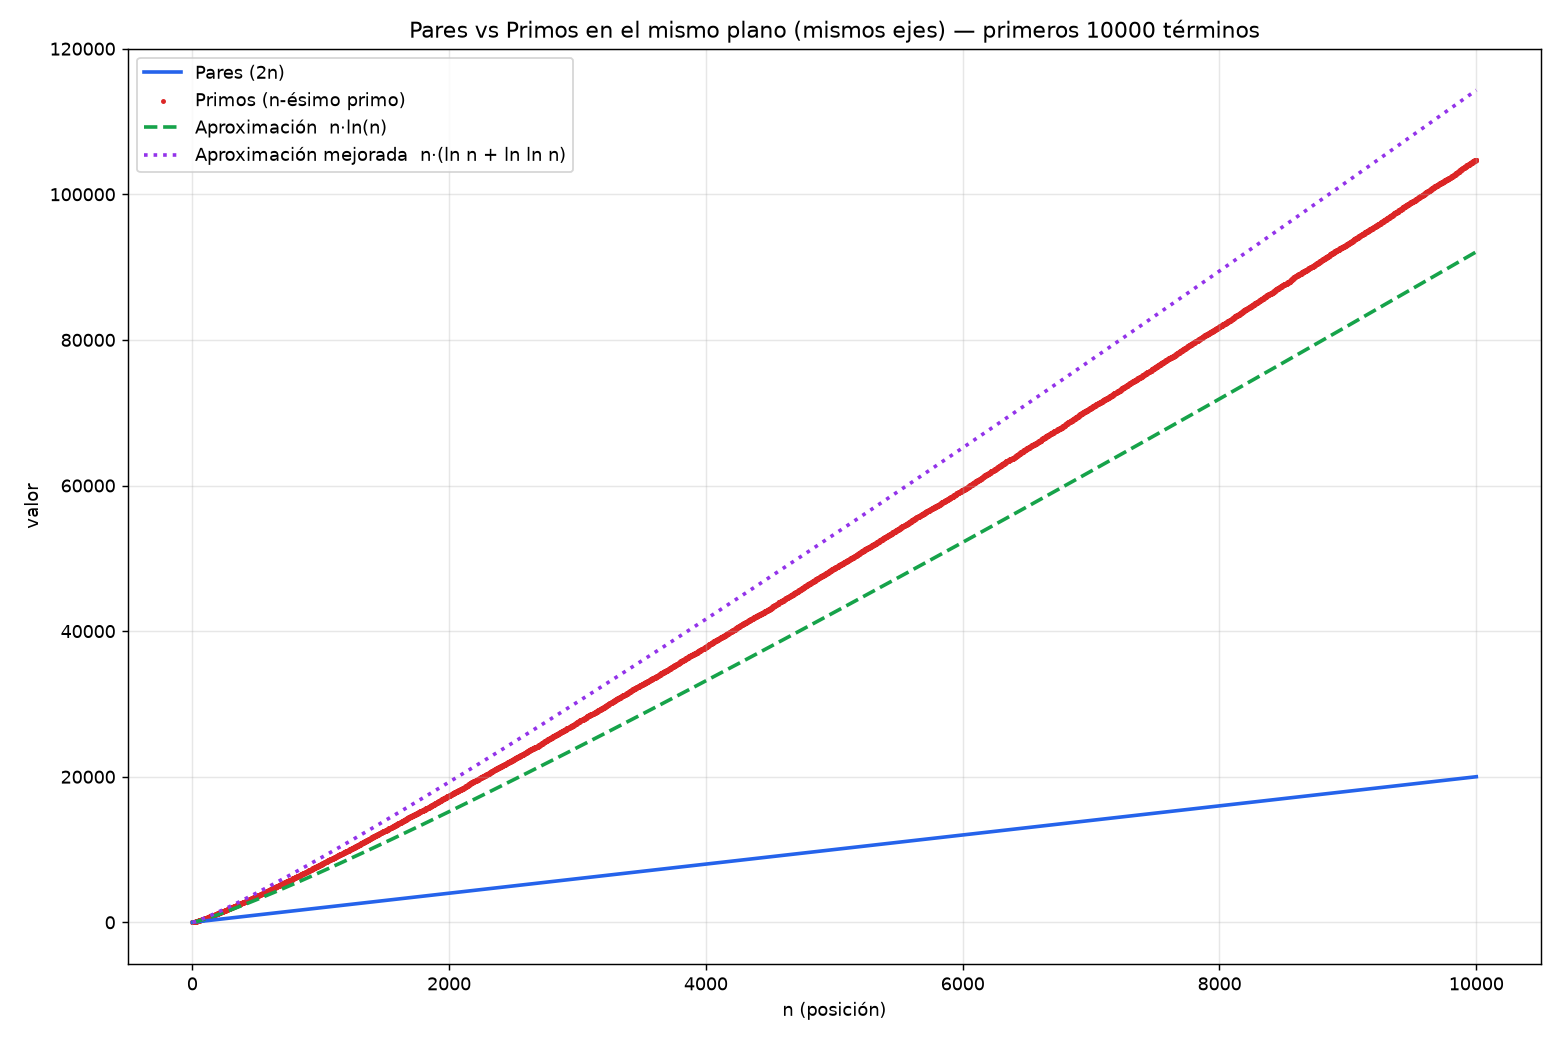
\includegraphics[width=0.92\textwidth]{sucesiones_comparacion.png}
  \caption{Pares, primos y las dos aproximaciones teóricas en el mismo plano. La
  recta azul (pares) queda aplastada abajo; los primos (rojo) quedan abrazados
  por las cotas verde y violeta.}
  \label{fig:comparacion}
\end{figure}

\section{La conexión con los primos: $\pi(x)$ frente a $\mathrm{Li}(x)$}

Para conectar los primos con la función zeta necesitamos la función contadora
$\pi(x)$ = cantidad de primos $\le x$, y su mejor aproximación suave, la
\textbf{integral logarítmica}:
\[
  \mathrm{Li}(x) = \int_2^x \frac{dt}{\ln t}.
\]

La Figura~\ref{fig:pi_li} (panel superior) muestra que $\mathrm{Li}(x)$ se pega
casi perfectamente a $\pi(x)$, mientras que la aproximación simple $x/\ln x$ se
queda corta. Pero lo importante está en el panel inferior: el \textbf{error}
$\pi(x)-\mathrm{Li}(x)$ oscila de forma irregular y queda \emph{atrapado} dentro
de una banda que crece como $\sqrt{x}$.

\begin{figure}[h]
  \centering
  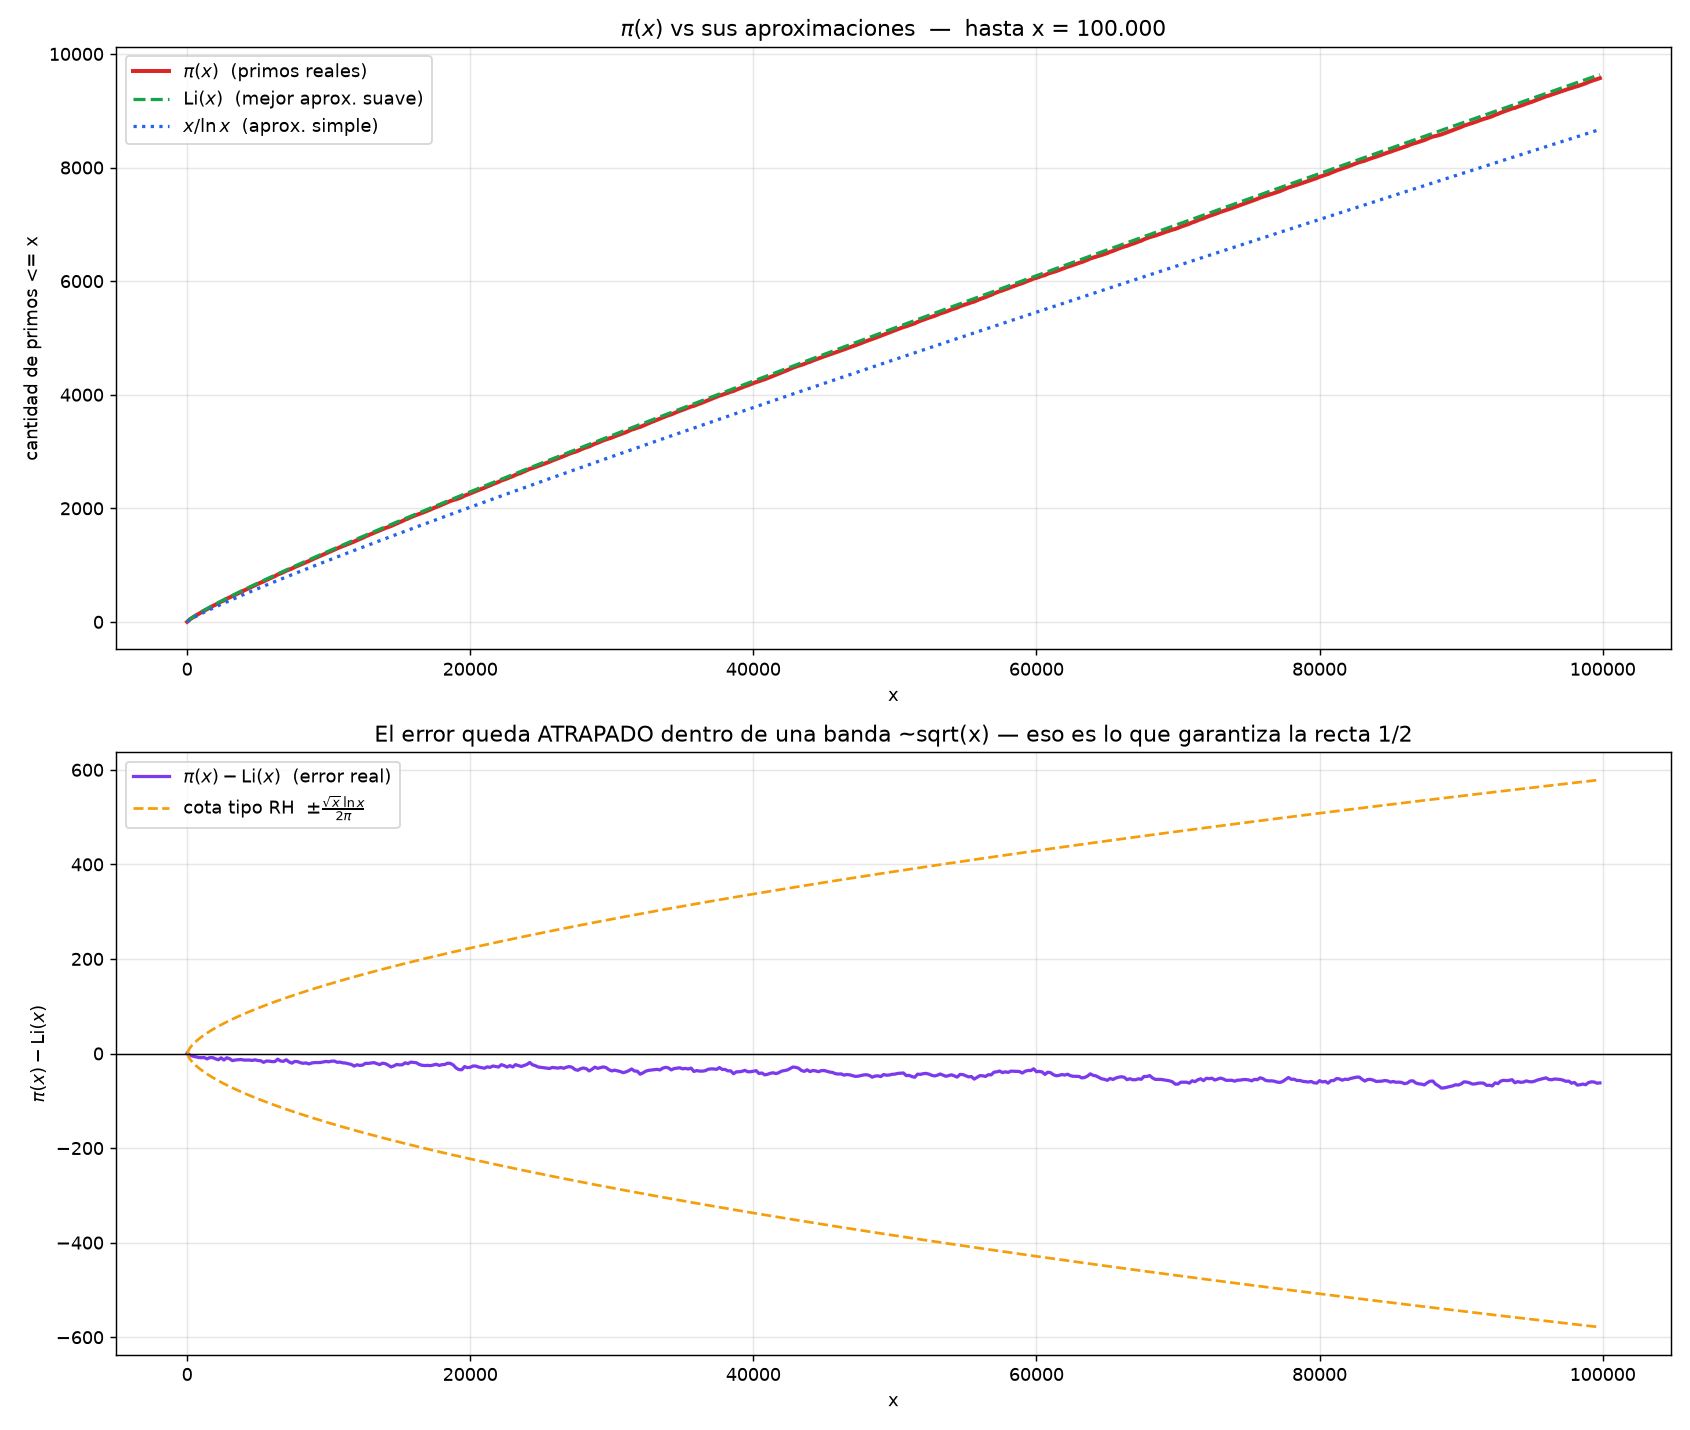
\includegraphics[width=0.95\textwidth]{pi_vs_li.png}
  \caption{Arriba: $\pi(x)$, $\mathrm{Li}(x)$ y $x/\ln x$. Abajo: el error
  $\pi(x)-\mathrm{Li}(x)$ oscilando dentro de una banda $\sim\sqrt{x}$.}
  \label{fig:pi_li}
\end{figure}

\begin{quote}
\textbf{Aquí aparece el $1/2$.} La Hipótesis de Riemann equivale a decir que este
error nunca se escapa de la banda $\sqrt{x}=x^{1/2}$. Ese exponente $\tfrac12$
es \emph{el mismo} $\tfrac12$ de la recta crítica. Si un solo cero se saliera a
$\mathrm{Re}(s)=0.6$, el error crecería como $x^{0.6}$ y rompería la banda.
\end{quote}

\section{La analogía de Barkhausen}

\subsection{Los ceros como modos de un oscilador}

La \textbf{fórmula explícita} (Sección~\ref{sec:explicita}) expresa el conteo de
primos como una suma de términos $x^\rho$, uno por cada cero $\rho=\beta+i\gamma$.
Con el cambio $x=e^u$ (es decir $u=\ln x$):
\[
  x^\rho = x^\beta \cdot x^{i\gamma}
         = \underbrace{e^{\beta u}}_{\text{envolvente}}\cdot
           \underbrace{e^{i\gamma u}}_{\text{oscilación}}.
\]

Esto es exactamente un \emph{modo} de un sistema lineal $e^{\sigma t}e^{i\omega t}$,
con tasa de crecimiento $\sigma=\beta$ y frecuencia $\omega=\gamma$. Normalizando
por el término dominante $\sqrt{x}=x^{1/2}$:
\[
  \frac{x^\beta}{x^{1/2}} = x^{\beta-1/2} = e^{(\beta-\frac12)u}.
\]

\begin{center}
\begin{tabular}{ll}
  \hline
  Posición del cero & Régimen \\
  \hline
  $\beta > 1/2$ & envolvente crece $\Rightarrow$ \textbf{diverge} (inestable)\\
  $\beta < 1/2$ & envolvente decae $\Rightarrow$ \textbf{muere} (sobreamortiguado)\\
  $\beta = 1/2$ & envolvente constante $\Rightarrow$ \textbf{oscilación sostenida}\\
  \hline
\end{tabular}
\end{center}

La condición $\beta=1/2$ es exactamente la \textbf{condición de Barkhausen} de un
oscilador: ganancia de lazo de módulo $1$, ni crecimiento ni decaimiento. La
Figura~\ref{fig:barkhausen} lo ilustra con la frecuencia del primer cero real,
$\gamma=14.1347\ldots$

\begin{figure}[h]
  \centering
  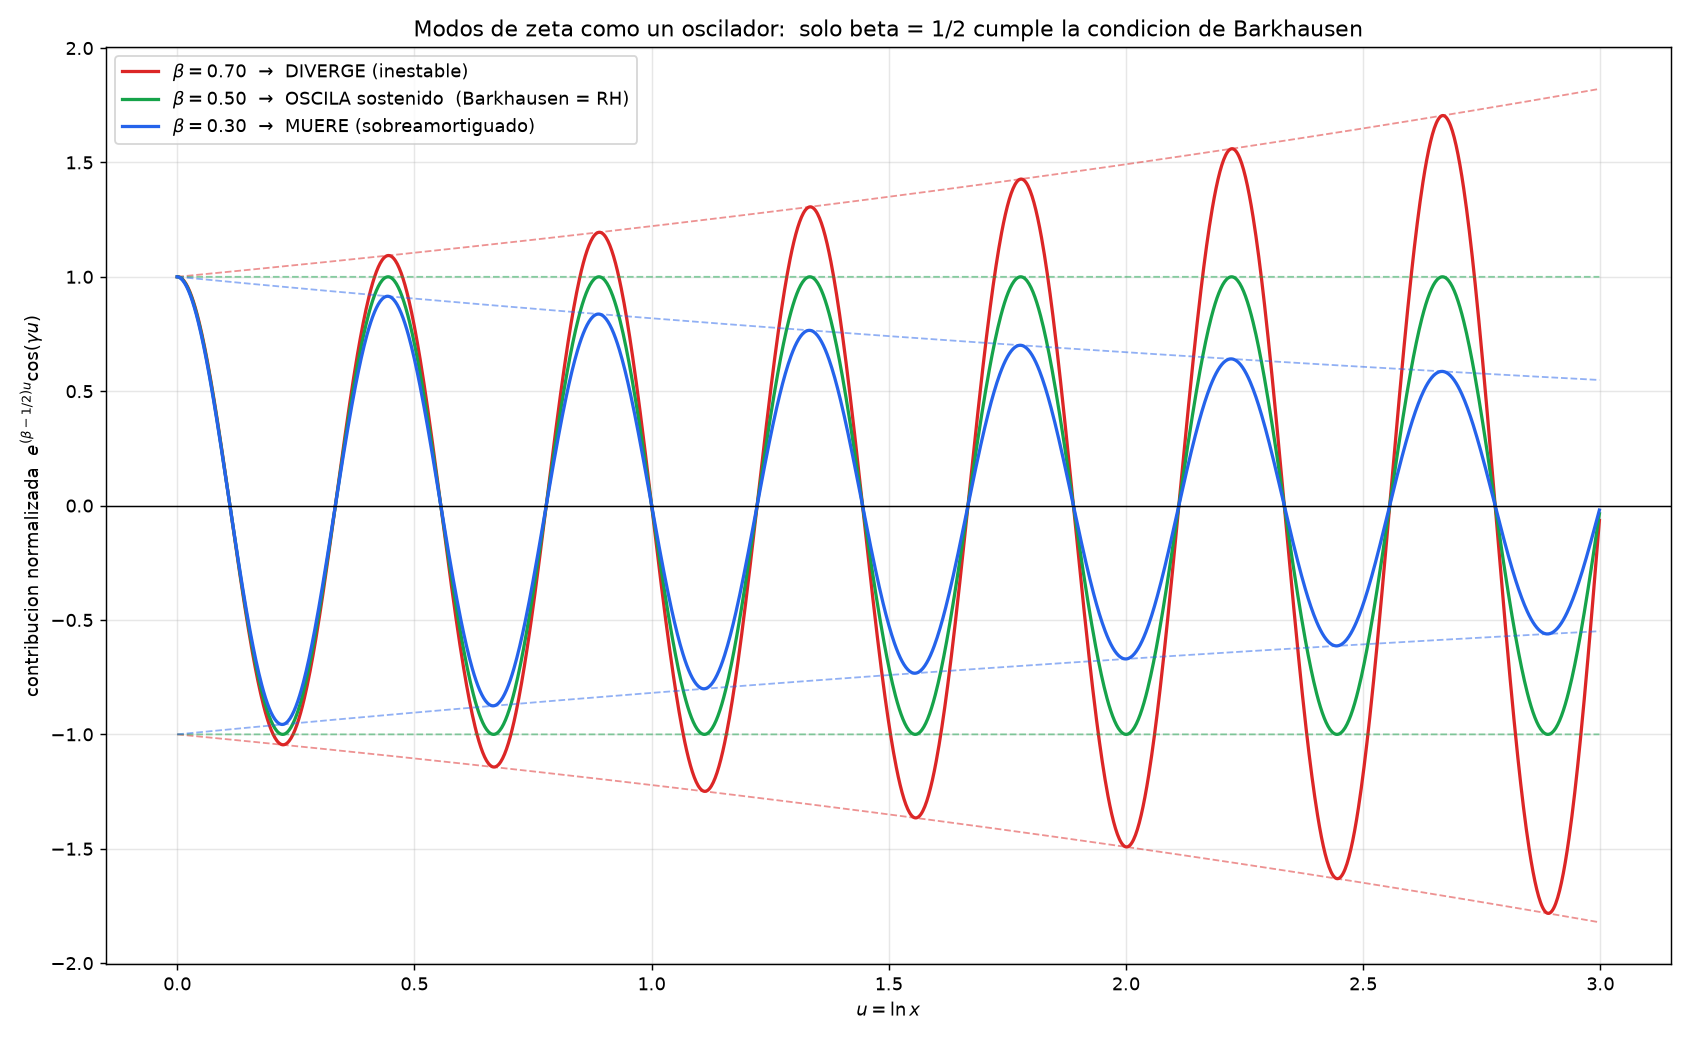
\includegraphics[width=0.92\textwidth]{barkhausen_riemann.png}
  \caption{El modo $e^{(\beta-1/2)u}\cos(\gamma u)$ para tres posiciones del cero.
  Solo $\beta=1/2$ (verde) tiene envolvente plana: oscilación sostenida.}
  \label{fig:barkhausen}
\end{figure}

\subsection{Qué es lo que oscila: un fasor de módulo 1}

La oscilación entre $+1$ y $-1$ es la proyección (parte real) de un fasor
$e^{i\gamma u}=\cos(\gamma u)+i\sin(\gamma u)$ que gira sobre el círculo
unitario. Su módulo es \emph{exactamente} $1$:
\[
  \bigl|e^{i\gamma u}\bigr| = 1.
\]
Ese módulo unitario \emph{es} la ganancia de lazo de Barkhausen, y solo se cumple
cuando $\beta=1/2$. La amplitud no crece ni muere porque, en el filo marginal,
la energía por ciclo se conserva ---como un oscilador $LC$ ideal sin resistencia.

\section{Zeta como forma de onda}

Sobre la recta crítica, la función $Z(t)$ de Riemann--Siegel es \emph{real} y
cumple $|Z(t)|=|\zeta(\tfrac12+it)|$. Es, literalmente, la forma de onda del
oscilador de zeta: cruza cero exactamente en cada cero
$\gamma=14.13,\,21.02,\,25.01,\dots$ (Figura~\ref{fig:zeta}, panel superior).

El panel inferior compara $|\zeta(\sigma+it)|$ para $\sigma=0.3,\,0.5,\,0.7$.
\textbf{Solo en $\sigma=1/2$ la curva toca el cero} (mínimo $0.001$ frente a
$0.17$ y $0.15$ en las otras rectas): la resonancia perfecta ocurre únicamente
sobre la recta crítica.

\begin{figure}[h]
  \centering
  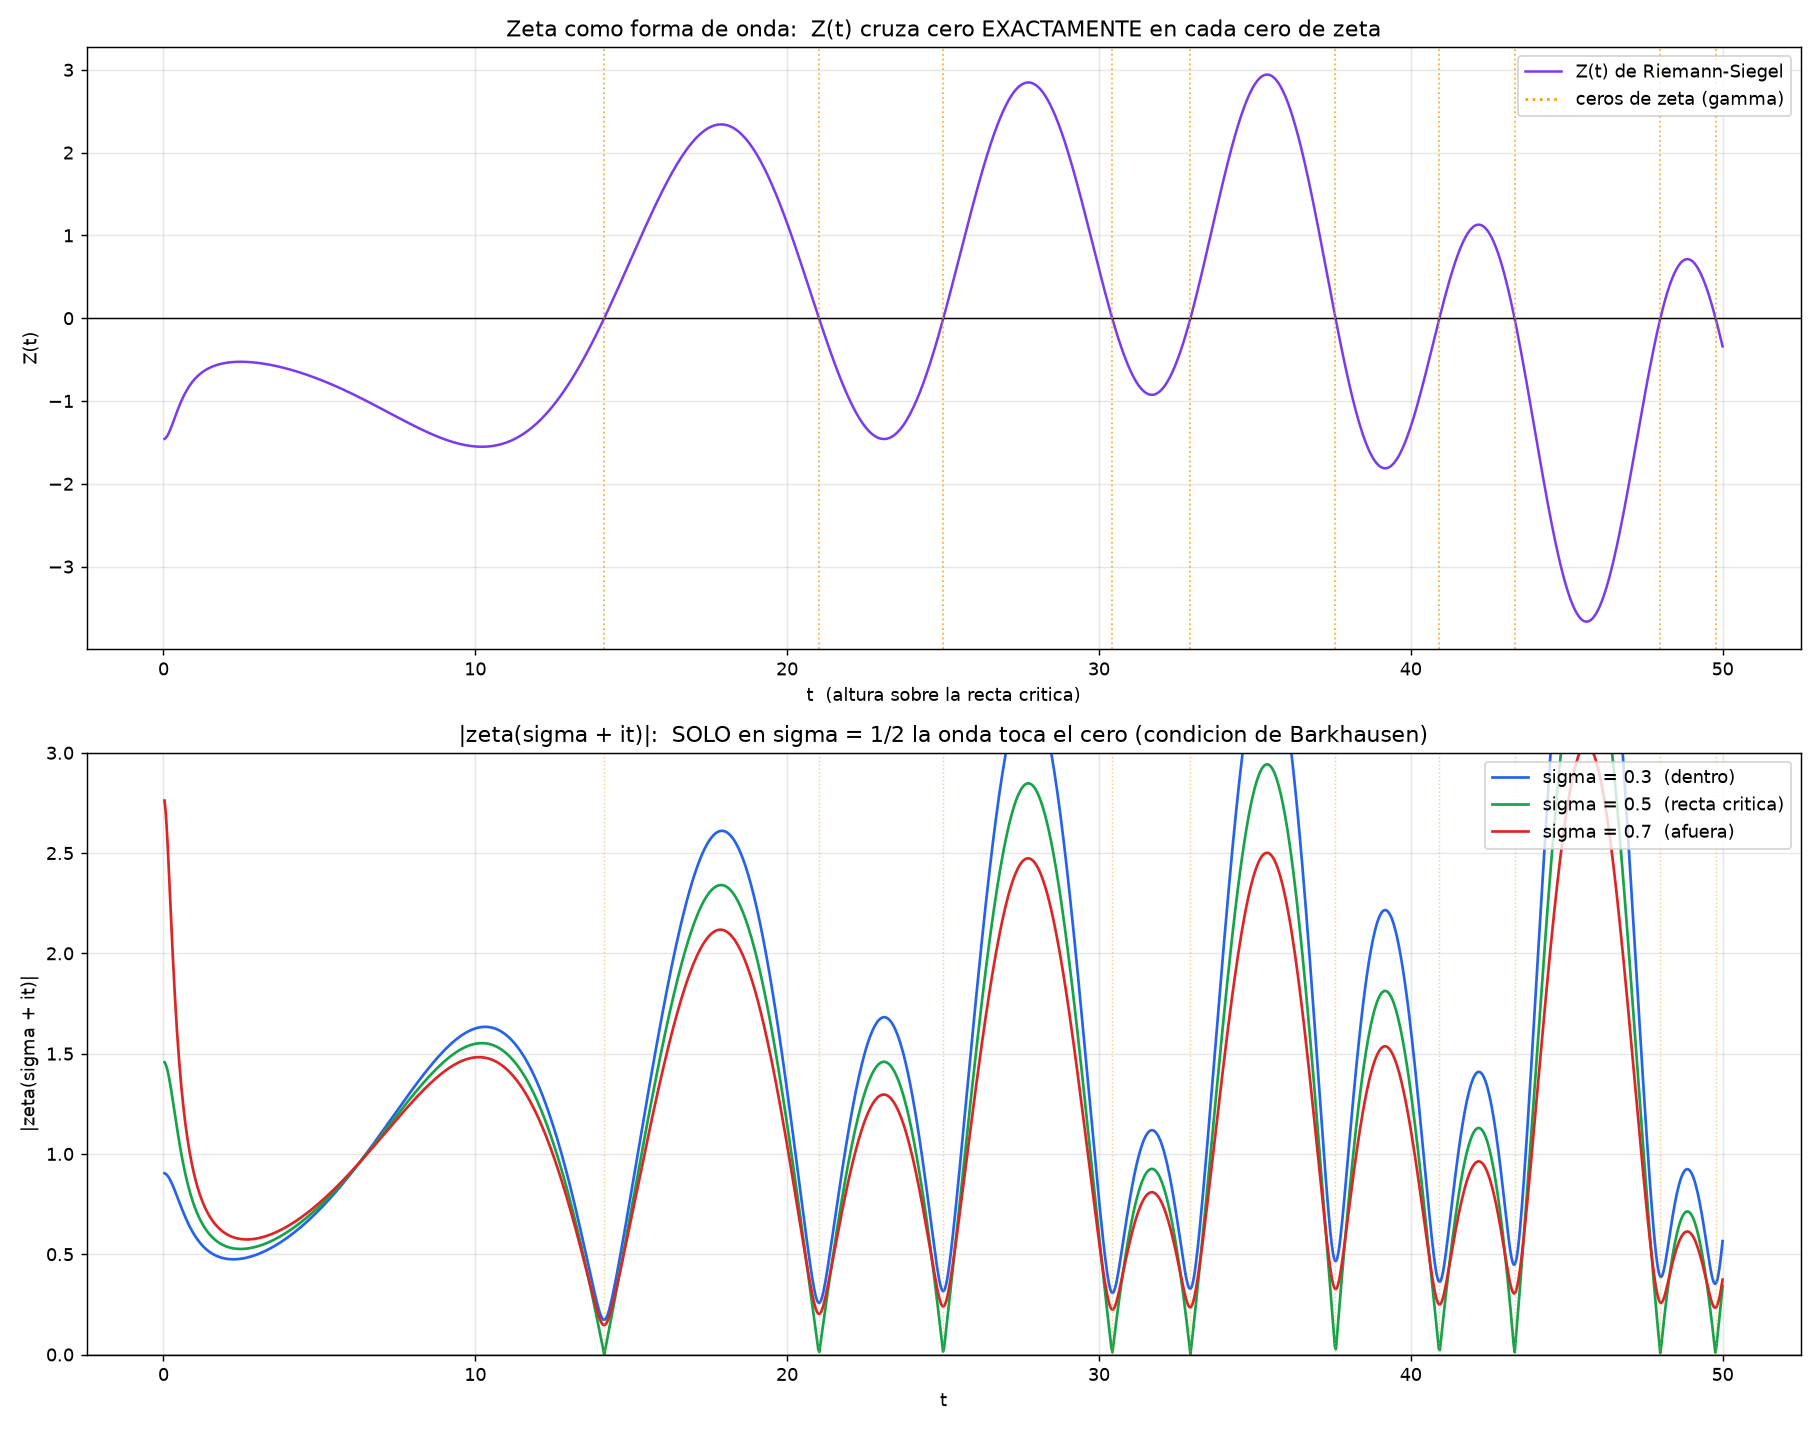
\includegraphics[width=0.9\textwidth]{zeta_barkhausen.png}
  \caption{Arriba: $Z(t)$ cruza cero en cada cero de zeta. Abajo: solo
  $\sigma=1/2$ hace que $|\zeta|$ toque cero (condición de Barkhausen).}
  \label{fig:zeta}
\end{figure}

\subsection{Comportamiento a gran altura ($t$ hasta $100.000$)}

Hasta $t=100.000$ hay unos $138.000$ ceros, demasiados para trazar la onda
completa. La Figura~\ref{fig:cien_mil} muestra el patrón global (conteo $N(t)$ y
espaciado medio $2\pi/\ln(t/2\pi)$) junto con cuatro ventanas-zoom de la onda
real. Observación clave: \textbf{la onda sigue siendo marginal en todas las
alturas} ---oscila cruzando cero, sin converger ni divergir--- pero la frecuencia
aumenta lentamente (el espaciado cae de $2.27$ en $t\approx100$ a $0.65$ en
$t\approx100.000$).

\begin{figure}[h]
  \centering
  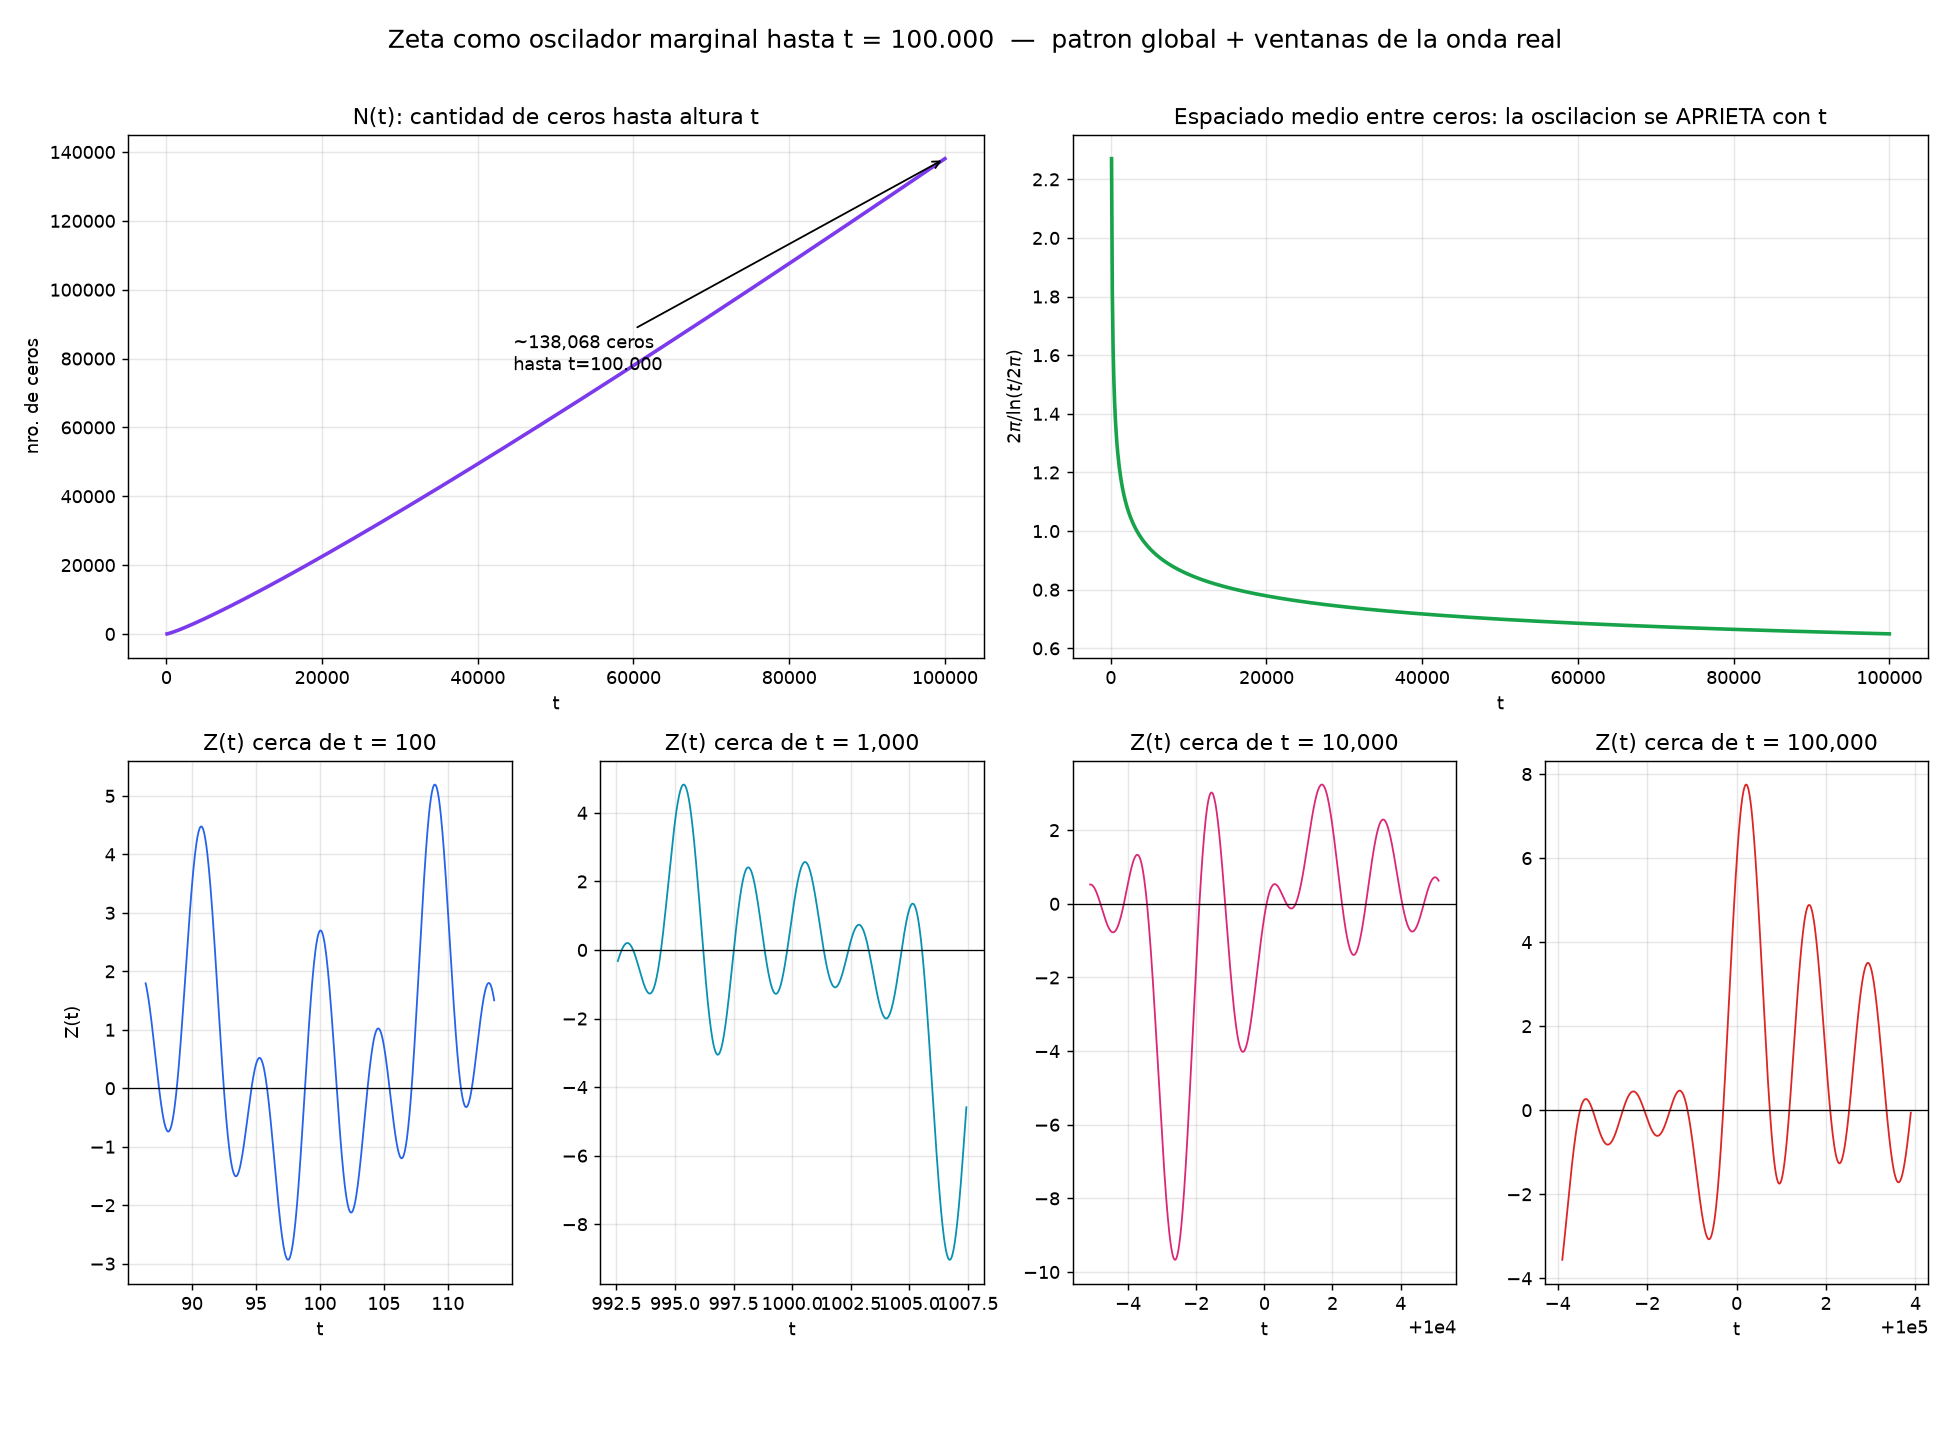
\includegraphics[width=0.97\textwidth]{zeta_barkhausen_100k.png}
  \caption{Patrón global hasta $t=100.000$ (fila superior) y ventanas de la onda
  $Z(t)$ a alturas crecientes (fila inferior). La marginalidad se mantiene en las
  $138.000$ oscilaciones.}
  \label{fig:cien_mil}
\end{figure}

\begin{quote}
\textbf{Que las curvas no converjan ni diverjan es la clave.} Al estar sobre la
recta $1/2$, estamos parados justo en el filo marginal; la envolvente es plana
por construcción. La convergencia o divergencia solo aparecería si nos moviéramos
fuera de la recta.
\end{quote}

\section{Dos poblaciones, dos rectas}

Es tentador pensar que los primos ``caen'' sobre la recta $1/2$. No es así: los
primos (y los pares) son \emph{números reales}, y viven sobre el eje horizontal.
Los ceros de zeta son \emph{números complejos} $\tfrac12\pm i\gamma$ y viven sobre
la recta vertical $\mathrm{Re}(s)=1/2$. La Figura~\ref{fig:plano} los muestra
juntos: dos ``cruces'' perpendiculares de puntos.

\begin{figure}[h]
  \centering
  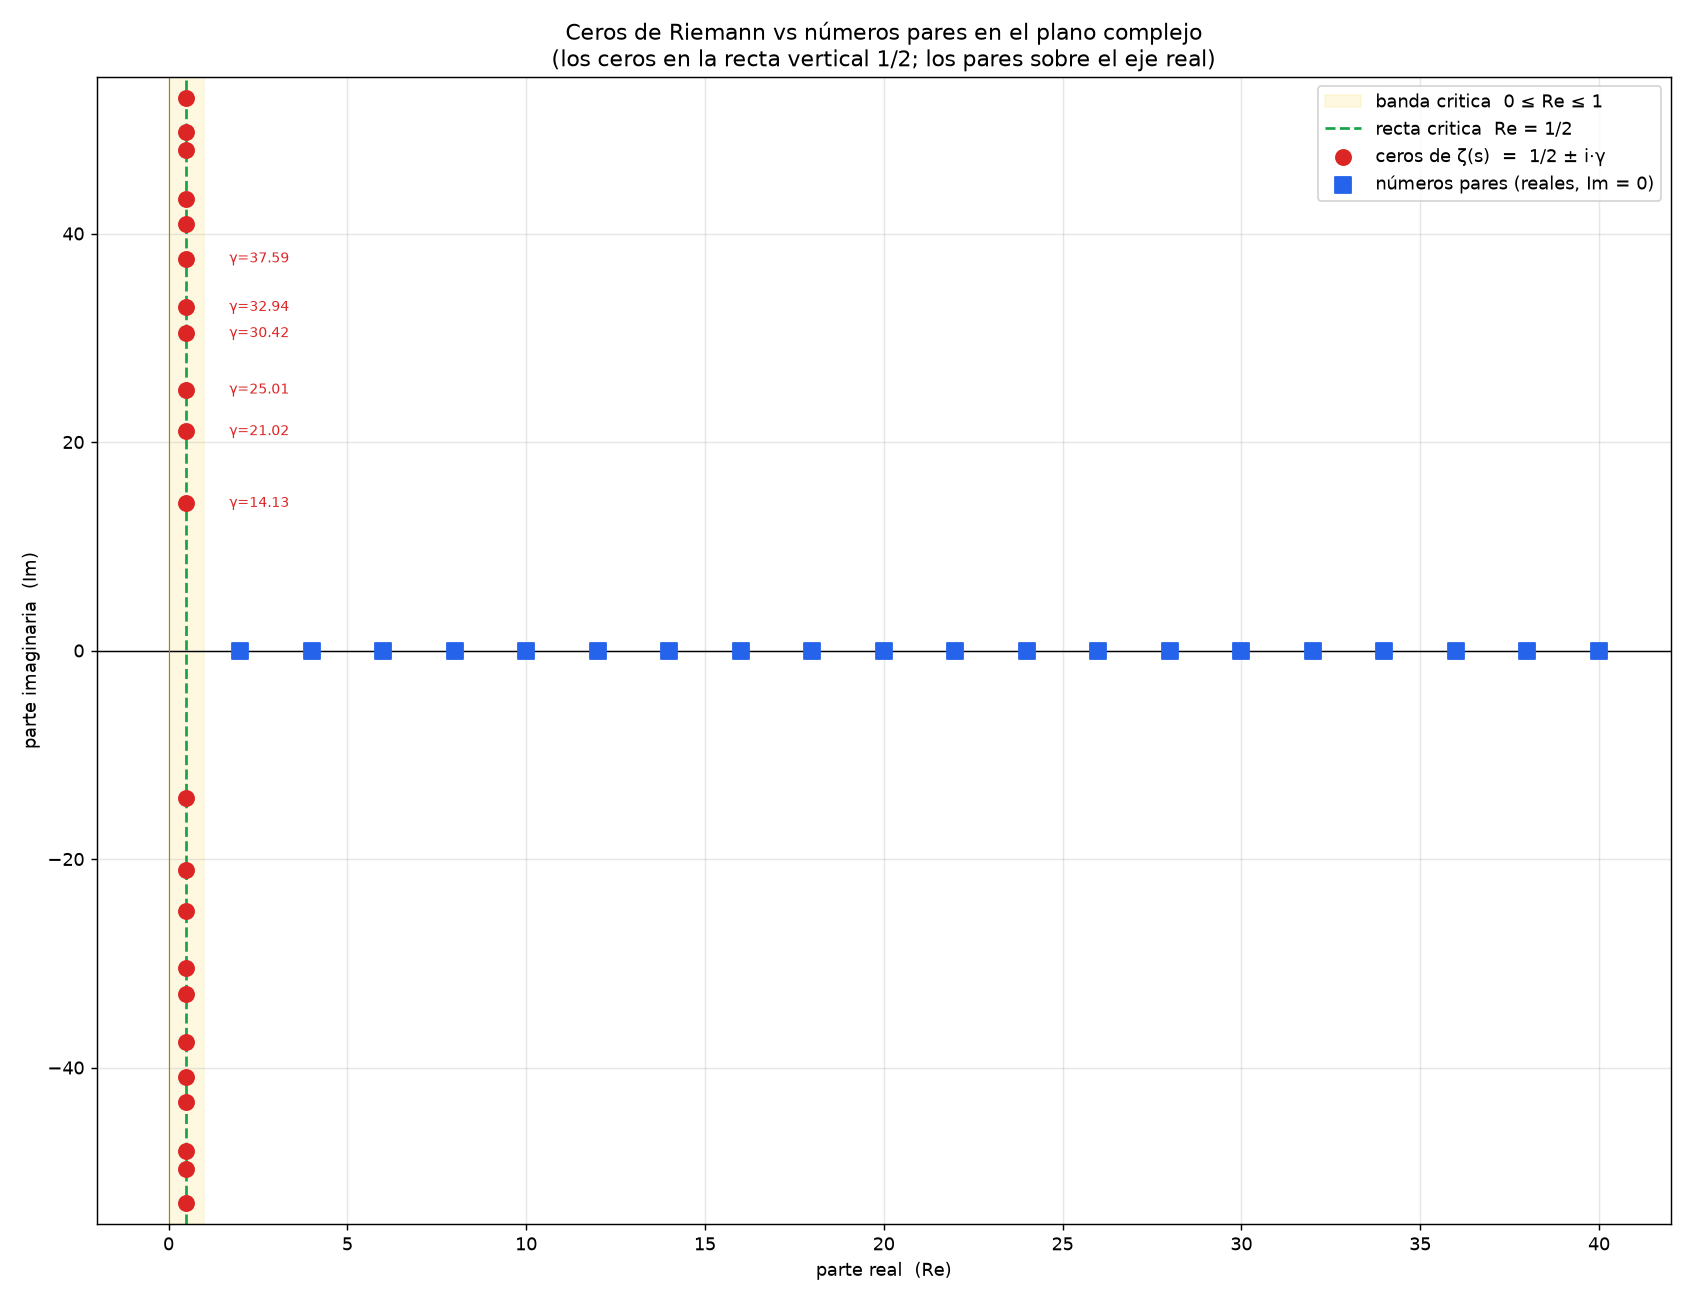
\includegraphics[width=0.85\textwidth]{ceros_vs_pares_plano.png}
  \caption{Los primeros $20$ ceros de zeta (rojo, sobre la recta vertical $1/2$)
  y los primeros $20$ pares (azul, sobre el eje real). Objetos de naturaleza
  distinta, en direcciones perpendiculares del plano.}
  \label{fig:plano}
\end{figure}

\begin{center}
\begin{tabular}{lll}
  \hline
   & Números pares & Ceros de zeta \\
  \hline
  Naturaleza & reales & complejos \\
  Dónde viven & eje real (horizontal) & recta $1/2$ (vertical) \\
  Espaciado & regular (trivial) & irregular (profundo) \\
  Fórmula & $2n$, exacta & sin fórmula cerrada \\
  \hline
\end{tabular}
\end{center}

\section{La fórmula explícita: los ceros reconstruyen a los primos}
\label{sec:explicita}

¿Cómo puede una lista de puntos sobre la recta vertical tener que ver con los
primos, que viven sobre el eje real? La respuesta es la \textbf{fórmula explícita
de Riemann}. Usando la función escalón de Chebyshev $\psi(x)$, que salta $\ln p$
en cada potencia de primo $p^k$:
\[
  \psi(x) = x - \sum_{\rho} \frac{x^\rho}{\rho} - \ln(2\pi)
            - \tfrac12\ln\!\left(1-x^{-2}\right).
\]

Cada cero $\rho=\tfrac12+i\gamma$ aporta una onda $x^\rho=\sqrt{x}\,e^{i\gamma\ln x}$
de frecuencia $\gamma$. Sumando más y más ondas, la reconstrucción se acerca a la
escalera dentada de los primos (Figura~\ref{fig:explicita}): con $1$ cero, una
onda suave; con $50$ ceros, los escalones aparecen \emph{exactamente} sobre
$2,3,4,5,7,8,9,11,\dots$

\begin{figure}[h]
  \centering
  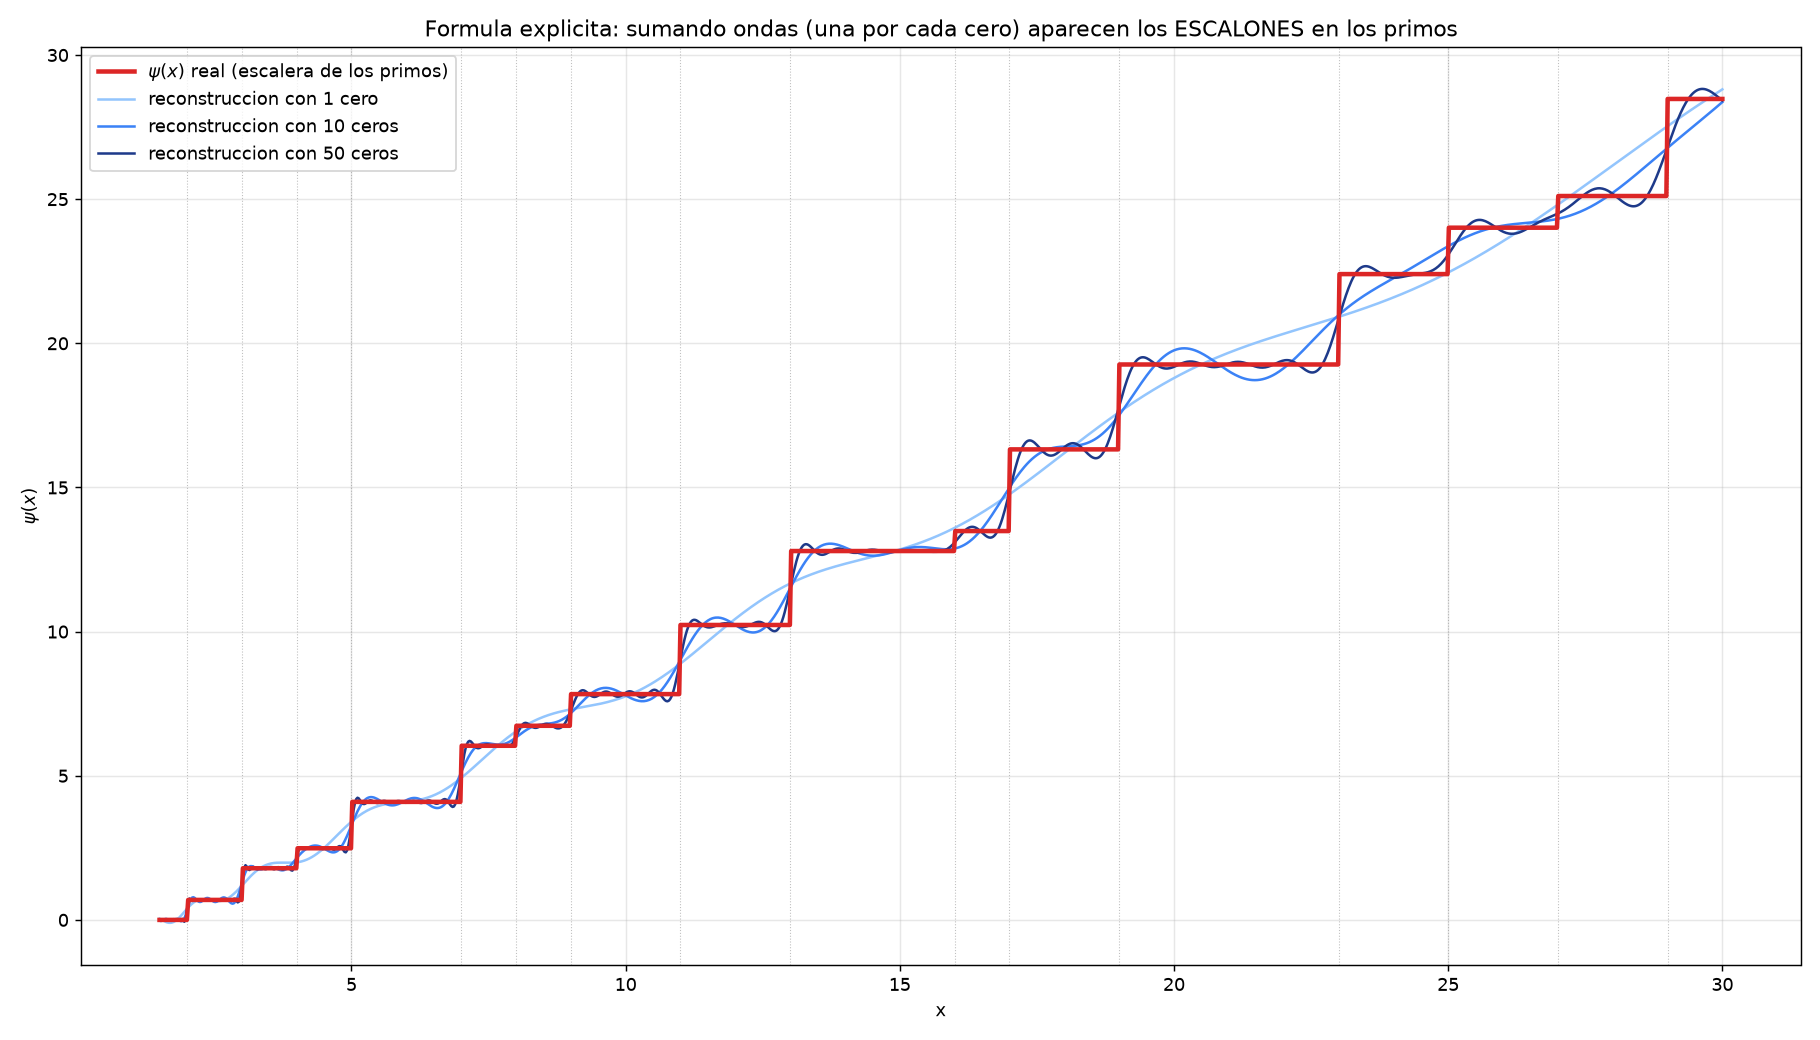
\includegraphics[width=0.95\textwidth]{formula_explicita.png}
  \caption{La escalera roja $\psi(x)$ codifica a los primos. Las curvas azules la
  reconstruyen usando solo los ceros de zeta: cuantos más ceros, más nítidos los
  escalones.}
  \label{fig:explicita}
\end{figure}

\begin{quote}
\textbf{Analogía musical.} La escalera de los primos es un acorde; los ceros de
zeta son las frecuencias puras (las notas) que, sumadas, lo producen. Los primos
no están \emph{sobre} la recta $1/2$: están \emph{codificados por} los puntos de
la recta $1/2$. La recta vertical es el espectro de frecuencias; el eje real es
donde suena la música.
\end{quote}

Como $|x^\rho|=x^{\mathrm{Re}(\rho)}=x^{1/2}$, todas las ondas tienen la misma
amplitud $\sqrt{x}$ ---\emph{precisamente porque} todos los ceros están en
$\mathrm{Re}=1/2$. Ese equilibrio (ninguna nota más fuerte que otra) es lo que
mantiene a los primos tan regulares como es posible. Es, una vez más, la condición
de Barkhausen: todas las ondas marginales, ninguna dominando.

\section{Cierre}

El recorrido completo ---pares $\to$ primos $\to$ $\pi(x)$ vs $\mathrm{Li}(x)$
$\to$ ceros $\to$ Barkhausen $\to$ fórmula explícita--- muestra que la Hipótesis
de Riemann es una afirmación sobre primos \emph{disfrazada} de afirmación sobre
ceros. En lenguaje de oscilador:

\begin{quote}
\emph{La función zeta mantiene la condición de estabilidad marginal (Barkhausen)
para sus infinitos ceros, de forma exacta y sin ningún mecanismo de control
visible.} La pregunta abierta es qué operador autoadjunto ---en el espíritu de
Hilbert--Pólya--- haría de ``control automático de ganancia'' que fuerza a cada
cero a quedarse clavado en $\mathrm{Re}(s)=1/2$.
\end{quote}

\end{document}
